\documentclass[a3paper,12pt]{extarticle} % Use extarticle for A3 paper size
\usepackage{graphicx} % Include this package for \includegraphics
\usepackage{amsmath}
\usepackage{amssymb} % Include this package for \mathbb
\usepackage[margin=1in]{geometry} % Adjust the margin as needed
\usepackage{float} % Include this package for the H float option

\begin{document}

\author{kipngeno koech - bkoech}
\title{Homework 4 - Introduction to Machine Learning for Engineers}   
\maketitle

\medskip

\maketitle

\section{Distributed SGD [20 points]}
Consider that we have a system of $m$ worker nodes and a parameter server performing distributed SGD (stochastic gradient descent). In each iteration, every worker node receives the model from the parameter server, computes one gradient step of the objective function locally using its local data, and sends the gradient to the parameter server. The parameter server does the aggregation of gradients using either synchronous SGD or asynchronous SGD.

The gradient calculation time $X_i$ taken by each node $i$ follows the exponential distribution with rate $\lambda = 2$, which has the following probability density function (PDF):
\begin{align}
f_X(x) = 
\begin{cases}
\lambda e^{-\lambda x} & \text{if } x \geq 0\\
0 & \text{else}
\end{cases}
\end{align}

Answer the following questions and make sure to explain your answers:

\begin{enumerate}
\item
What is the cumulative distribution function (CDF) of $f_X(x)$, i.e., $F_X(x)$?
\\ We find the CDF by integrating the PDF:
\begin{align}
F_X(x) &= \int_{-\infty}^x f_X(t) dt\\
&= \int_{0}^x \lambda e^{-\lambda t} dt\\
&= \left[-e^{-\lambda t}\right]_{0}^x\\
&= -e^{-\lambda x} + 1\\
&= 1 - e^{-\lambda x}
\end{align}
integrating from $0$ to $x$ since the PDF is $0$ for $x < 0$.

\begin{align}
F_X(x) =
\begin{cases}
0 & \text{if } x < 0\\
1 - e^{-\lambda x} & \text{if } x \geq 0
\end{cases}
\end{align}

\item
Define $X_{m:m}$ as the maximum of $m$ i.i.d. (independently and identically distributed) instances $X_1, ..., X_m$ following the distribution $X$. What is the CDF of $X_{m:m}$, and what is the expected value $E[X_{m:m}]$?
\\ The CDF of the maximum of $m$ i.i.d. random variables is given by:
\begin{align}
F_{X_{m:m}}(x) = P(X_{m:m} \leq x) = P(X_1 \leq x, X_2 \leq x, ..., X_m \leq x) = P(X \leq x)^m = (F_X(x))^m
\end{align}
Substituting the CDF we found in part (a):
\begin{align}
F_{X_{m:m}}(x) =
\begin{cases}
0 & \text{if } x < 0\\
(1 - e^{-\lambda x})^m & \text{if } x \geq 0
\end{cases}
\end{align}
To find the expected value $E[X_{m:m}]$, we can use the following formula:
\begin{align}
E[X_{m:m}] = \int_0^\infty (1 - F_{X_{m:m}}(x)) dx
&= \int_0^\infty (1 - (1 - e^{-\lambda x})^m) dx\\
\end{align}
We need to evaluate this integral. We can use integration by parts or numerical methods to find the expected value. The result is:
\begin{align}
E[X_{m:m}] = \frac{1}{\lambda} \sum_{k=1}^m \frac{1}{k}
\end{align}
This is the expected value of the maximum of $m$ i.i.d. exponential random variables with rate $\lambda$.


\item
Define $X_{1:m}$ as the minimum of $m$ i.i.d instances $X_1, ..., X_m$ following the distribution $X$. What is the CDF of $X_{1:m}$, and what is the expected value $E[X_{1:m}]$?
\\ The CDF of the minimum of $m$ i.i.d. random variables is given by:
\begin{align}
F_{X_{1:m}}(x) = P(X_{1:m} \leq x) = P(X_1 \leq x, X_2 \leq x, ..., X_m \leq x) = 1 - P(X > x)^m = 1 - (1 - F_X(x))^m
\end{align}
Substituting the CDF:
\begin{align}
F_{X_{1:m}}(x) =
\begin{cases}
0 & \text{if } x < 0\\
1 - (e^{-\lambda x})^m & \text{if } x \geq 0
\end{cases}
\end{align}
To find the expected value $E[X_{1:m}]$, we can use the following formula:
\begin{align}
E[X_{1:m}] = \int_0^\infty (1 - F_{X_{1:m}}(x)) dx
&= \int_0^\infty (e^{-\lambda x})^m dx\\
&= \int_0^\infty e^{-m\lambda x} dx\\
&= \frac{1}{m\lambda}
\end{align}
This is the expected value of the minimum of $m$ i.i.d. exponential random variables with rate $\lambda$.


\item
In this sub-problem, we will simulate and compare the expected runtime per iteration of synchronous SGD and asynchronous SGD for different values of $m$. The time for each worker node to finish one gradient computation is exponentially distributed as given in part (a) with $\lambda = 2$, and it is i.i.d. across workers and iterations. Assume there is no communication delay.

Simulate 5000 iterations of training using Python for different values of $m$ ranging from 1 to 20, and obtain the average runtime per iteration. Make a comparative plot of the average runtimes per iteration of synchronous and asynchronous SGD versus $m$. Explain the trends observed in the plot in 1-2 sentences. You may use packages inside \texttt{numpy.random} to draw random samples from the exponential distribution. Attach your plot and code in PDF format to the end of your homework.
\begin{figure}[h]
\centering
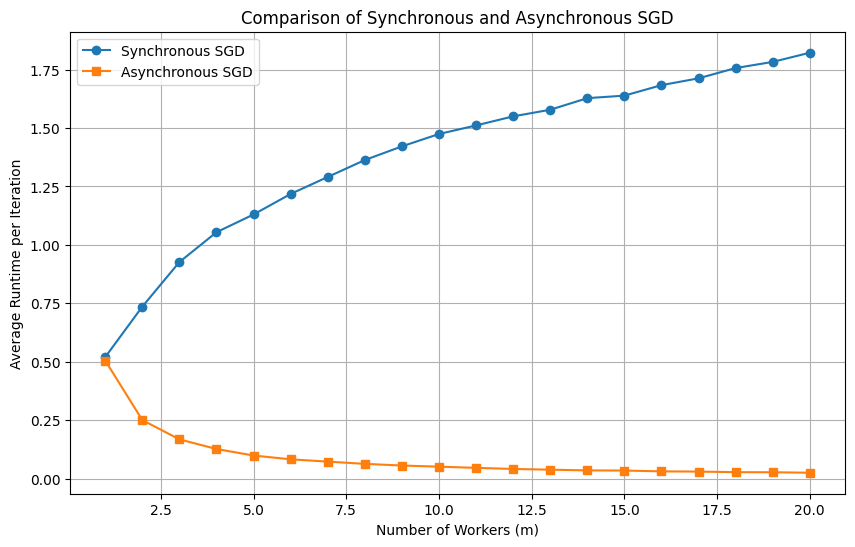
\includegraphics[width=0.8\textwidth]{asynchronousVsynchronous.png}
\caption{Average runtimes per iteration of synchronous and asynchronous SGD versus $m$.}
\end{figure}

The synchronous SGD takes the maximum time among all workers to finish their gradient computation, while the asynchronous SGD takes the minimum time. As $m$ increases, the average runtime of synchronous SGD increases due to the increased waiting time for the slowest worker, while the average runtime of asynchronous SGD decreases due to the increased probability of having at least one fast worker. This is reflected in the plot where the average runtime of synchronous SGD increases with $m$, while that of asynchronous SGD decreases.


\item
Write down the theoretical expressions for the expected runtimes per iteration of synchronous and asynchronous SGD in terms of $m$ and $\lambda$ (Hint: You can use the expressions derived in parts (b) and (c)). On the figure generated in part (d), also plot the theoretical expected runtimes versus $m$. Check whether the theoretical and simulated values align.
\begin{figure}
\centering
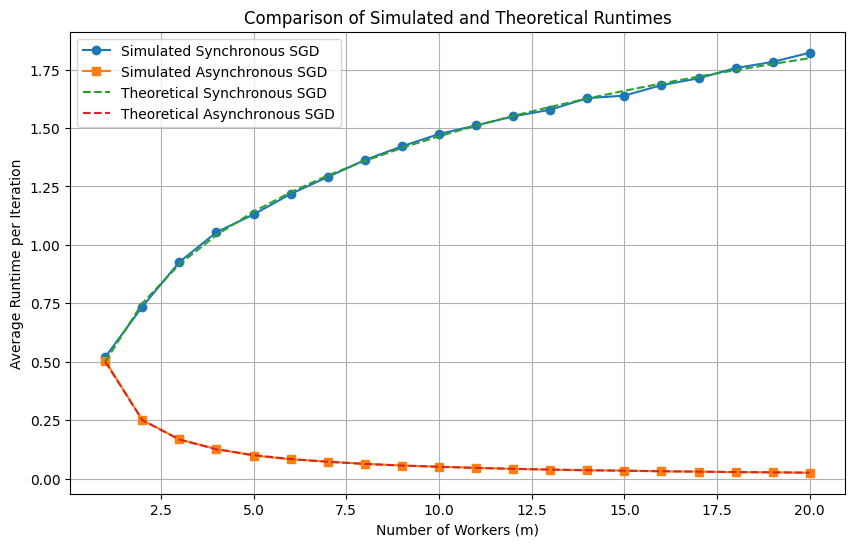
\includegraphics[width=0.8\textwidth]{theoriticalVPlotted.png}
\caption{Average runtimes per iteration of synchronous and asynchronous SGD versus $m$ with theoretical expected runtimes.}
\end{figure}
\end{enumerate}
The theoretical expected runtimes per iteration of synchronous and asynchronous SGD are given by:
\begin{align}
E[T_{sync}] &= \frac{1}{\lambda} \sum_{k=1}^m \frac{1}{k}\\
E[T_{async}] &= \frac{1}{m\lambda}
\end{align}
where $E[T_{sync}]$ is the expected runtime of synchronous SGD and $E[T_{async}]$ is the expected runtime of asynchronous SGD. The plot shows that the theoretical and simulated values align well, confirming the correctness of our theoretical expressions.

\newpage
\section{K-means [20 points]}

Given a set of data points $\{\mathbf{x}_n\}_{n=1}^N$, k-means clustering minimizes the following distortion measure (also called the ``objective'' or ``clustering cost''):
\begin{align}
D = \sum_{n=1}^N \sum_{k=1}^K r_{nk} \|\mathbf{x}_n - \boldsymbol{\mu}_k\|^2_2
\end{align}
where $\boldsymbol{\mu}_k$ is the prototype of the $k$-th cluster and $r_{nk}$ is a binary indicator variable. If $\mathbf{x}_n$ is assigned to the cluster $k$, $r_{nk}$ is 1, and otherwise $r_{nk}$ is 0. For each cluster, $\boldsymbol{\mu}_k$ is the prototype representative for all the data points assigned to that cluster.

\begin{enumerate}
    \item In lecture, we stated but did not prove that $\boldsymbol{\mu}_k$ is the mean of all points associated with the $k$th cluster, thus motivating the name of the algorithm. You will now prove this statement. Assuming all $r_{nk}$ are known (i.e., assuming you know the cluster assignments of all $N$ data points), show that the objective $D$ is minimized when each $\boldsymbol{\mu}_k$ is chosen as the mean of all data points assigned to cluster $k$, for any $k$. This justifies the iterative procedure of k-means\footnote{More rigorously, one would also need to show that if all $\boldsymbol{\mu}_k$ are known, then $r_{nk}$ can be computed by assigning $\mathbf{x}_n$ to the nearest $\boldsymbol{\mu}_k$. You are not required to do so.}.
\\
Let us denote the set of data points assigned to cluster $k$ as $C_k = \{n: r_{nk} = 1\}$. The objective function can be rewritten as:
\begin{align}
D &= \sum_{k=1}^K \sum_{n \in C_k} \|\mathbf{x}_n - \boldsymbol{\mu}_k\|^2_2\\
&= \sum_{k=1}^K \sum_{n \in C_k} \left( \|\mathbf{x}_n\|^2_2 - 2\mathbf{x}_n^T\boldsymbol{\mu}_k + \|\boldsymbol{\mu}_k\|^2_2 \right)\\
&= \sum_{k=1}^K \left( \sum_{n \in C_k} \|\mathbf{x}_n\|^2_2 - 2\boldsymbol{\mu}_k^T \sum_{n \in C_k} \mathbf{x}_n + |C_k| \|\boldsymbol{\mu}_k\|^2_2 \right)
\end{align}
where $|C_k|$ is the number of data points assigned to cluster $k$.
Now, we can differentiate $D$ with respect to $\boldsymbol{\mu}_k$ and set it to zero to find the optimal $\boldsymbol{\mu}_k$:
\begin{align}
\frac{\partial D}{\partial \boldsymbol{\mu}_k} &= -2 \sum_{n \in C_k} \mathbf{x}_n + 2|C_k|\boldsymbol{\mu}_k = 0\\
\sum_{n \in C_k} \mathbf{x}_n &= |C_k|\boldsymbol{\mu}_k\\
\boldsymbol{\mu}_k &= \frac{1}{|C_k|} \sum_{n \in C_k} \mathbf{x}_n
\end{align}
Thus, the optimal $\boldsymbol{\mu}_k$ is the mean of all data points assigned to cluster $k$.
    \item As discussed in lecture, sometimes we wish to scale each feature in order to ensure that ``larger'' features do not dominate the clustering. Suppose that each data point $\mathbf{x}_n$ is a $d$-dimensional feature vector and that we scale the $j$th feature by a factor $w_j > 0$. Letting $\mathbf{W}$ denote a $d \times d$ diagonal matrix with the $j$'th diagonal entry being $w_j$, $j = 1, 2, \ldots, d$, we can write our transformed features as $\mathbf{x}' = \mathbf{W}\mathbf{x}$.

Suppose we fix the $r_{nk}$, i.e., we take the assignment of data points $\mathbf{x}_n$ to clusters $k$ as given. Our goal is then to find the cluster centers $\boldsymbol{\mu}_k$ that minimize the distortion measure
\begin{align}
D = \sum_{n=1}^N \sum_{k=1}^K r_{nk} \|\mathbf{W}\mathbf{x}_n - \boldsymbol{\mu}_k\|^2_2.
\end{align}

Show that the cluster centers $\{\boldsymbol{\mu}_k\}$ that do so are given by $\boldsymbol{\mu}_k = \frac{1}{\sum_{n=1}^N r_{nk}} \mathbf{W} \sum_{n=1}^N r_{nk}\mathbf{x}_n$.
\\
Let us denote the set of data points assigned to cluster $k$ as $C_k = \{n: r_{nk} = 1\}$. The objective function can be rewritten as:
\begin{align}
D &= \sum_{k=1}^K \sum_{n \in C_k} \|\mathbf{W}\mathbf{x}_n - \boldsymbol{\mu}_k\|^2_2\\
&= \sum_{k=1}^K \sum_{n \in C_k} \left( \|\mathbf{W}\mathbf{x}_n\|^2_2 - 2(\mathbf{W}\mathbf{x}_n)^T\boldsymbol{\mu}_k + \|\boldsymbol{\mu}_k\|^2_2 \right)\\
&= \sum_{k=1}^K \left( \sum_{n \in C_k} \|\mathbf{W}\mathbf{x}_n\|^2_2 - 2\boldsymbol{\mu}_k^T \sum_{n \in C_k} \mathbf{W}\mathbf{x}_n + |C_k| \|\boldsymbol{\mu}_k\|^2_2 \right)
\end{align}
where $|C_k|$ is the number of data points assigned to cluster $k$.
Now, we can differentiate $D$ with respect to $\boldsymbol{\mu}_k$ and set it to zero to find the optimal $\boldsymbol{\mu}_k$:
\begin{align}
\frac{\partial D}{\partial \boldsymbol{\mu}_k} &= -2 \sum_{n \in C_k} \mathbf{W}\mathbf{x}_n + 2|C_k|\boldsymbol{\mu}_k = 0\\
\sum_{n \in C_k} \mathbf{W}\mathbf{x}_n &= |C_k|\boldsymbol{\mu}_k\\
\boldsymbol{\mu}_k &= \frac{1}{|C_k|} \sum_{n \in C_k} \mathbf{W}\mathbf{x}_n
\end{align}

We can rewrite the sum over $C_k$ as a sum over all points using the indicator variables $r_{nk}$, and note that $|C_k| = \sum_{n=1}^N r_{nk}$:
\begin{align}
\boldsymbol{\mu}_k &= \frac{1}{\sum_{n=1}^N r_{nk}} \sum_{n=1}^N r_{nk}\mathbf{W}\mathbf{x}_n
\end{align}

Since $\mathbf{W}$ is a diagonal matrix that doesn't depend on the summation index $n$, we can factor it out of the summation:
\begin{align}
\boldsymbol{\mu}_k &= \frac{1}{\sum_{n=1}^N r_{nk}}\mathbf{W}\sum_{n=1}^N r_{nk}\mathbf{x}_n
\end{align}

Thus, the cluster centers $\boldsymbol{\mu}_k$ that minimize the distortion measure are given by:
\begin{align}
\boldsymbol{\mu}_k = \frac{1}{\sum_{n=1}^N r_{nk}} \mathbf{W} \sum_{n=1}^N r_{nk}\mathbf{x}_n
\end{align}

\end{enumerate}
\newpage

\section{ 3-Dimensional Principal Component Analysis [20 points]}

In this problem, we will perform PCA on 3-dimensional data step by step. We are given three data points:
\begin{align}
\mathbf{x}_1 &= [0, -1, -2]\\
\mathbf{x}_2 &= [1, 1, 1]\\
\mathbf{x}_3 &= [2, 0, 1]
\end{align}

and we want to find 2 principal components of the given data.

\begin{enumerate}
\item First, find the covariance matrix $\mathbf{C}_X = \mathbf{X}^T \mathbf{X}$ where $\mathbf{X} = \begin{bmatrix} \mathbf{x}_1 - \bar{\mathbf{x}} \\ \mathbf{x}_2 - \bar{\mathbf{x}} \\ \mathbf{x}_3 - \bar{\mathbf{x}} \end{bmatrix}$, where $\bar{\mathbf{x}} = \frac{1}{3}(\mathbf{x}_1 + \mathbf{x}_2 + \mathbf{x}_3)$ is the mean of the data samples. Then, find the eigenvalues and the corresponding eigenvectors of $\mathbf{C}_X$. Feel free to use any numerical analysis program such as numpy, e.g., \texttt{numpy.linalg.eig} can be useful. However, you should explain what you inputted into this program.
\\ Finding the mean $\bar{\mathbf{x}}$:
\begin{align}
\bar{\mathbf{x}} &= \frac{1}{3}(\mathbf{x}_1 + \mathbf{x}_2 + \mathbf{x}_3)\\
&= \frac{1}{3}([0, -1, -2] + [1, 1, 1] + [2, 0, 1])\\
&= \frac{1}{3}([3, 0, 0])\\
&= [1, 0, 0]
\end{align}
let us find $\mathbf{X}$:
\begin{align}
\mathbf{X} &= \begin{bmatrix} \mathbf{x}_1 - \bar{\mathbf{x}} \\ \mathbf{x}_2 - \bar{\mathbf{x}} \\ \mathbf{x}_3 - \bar{\mathbf{x}} \end{bmatrix}\\
&= \begin{bmatrix} [0, -1, -2] - [1, 0, 0] \\ [1, 1, 1] - [1, 0, 0] \\ [2, 0, 1] - [1, 0, 0] \end{bmatrix}\\
&= \begin{bmatrix} [-1, -1, -2] \\ [0, 1, 1] \\ [1, 0, 1] \end{bmatrix}
\end{align}
Now, we can find the covariance matrix $\mathbf{C}_X$:
\begin{align}
\mathbf{C}_X &=  \mathbf{X}^T \mathbf{X}\\
&=  \begin{bmatrix} [-1, 0, 1] \\ [-1, 1, 0] \\ [-2, 1, 1] \end{bmatrix} \begin{bmatrix} [-1, -1, -2] \\ [0, 1, 1] \\ [1, 0, 1] \end{bmatrix}\\
&= \begin{bmatrix} 2 & 1 & 3 \\ 1 & 2 & 3 \\ 3 & 3 & 6 \end{bmatrix}
\end{align}
Now, we can find the eigenvalues and eigenvectors of $\mathbf{C}_X$ using numpy:
\begin{verbatim}
import numpy as np
C_X = np.array([[2, 1, 3], [1, 2, 3], [3, 3, 6]])
eigenvalues, eigenvectors = np.linalg.eig(C_X)
print("Eigenvalues:", eigenvalues)
print("Eigenvectors:", eigenvectors)
\end{verbatim}
The output will give us the eigenvalues and eigenvectors of the covariance matrix. The eigenvalues are:
\begin{align}
\lambda_1 &= 9.00\\
\lambda_2 &= 1.00\\
\lambda_3 &= 0.00
\end{align}
The corresponding eigenvectors are:
\begin{align}
    \mathbf{u}_1  &= \begin{pmatrix}
    1\\
    1\\
    2
    \end{pmatrix}
    \mathbf{u}_2  &= \begin{pmatrix}
    -1\\
    1\\
    0
    \end{pmatrix}
    \mathbf{u}_3  &= \begin{pmatrix}
    -1\\
    -1\\
    1
    \end{pmatrix}
\end{align}
I used the numpy function \texttt{numpy.linalg.eig} to compute the eigenvalues and eigenvectors of the covariance matrix. The input to this function was the covariance matrix $\mathbf{C}_X$ that we computed above.   
\item 
Using the result above, find the first two principal components of the given data.
\\ The first two principal components are the eigenvectors corresponding to the two largest eigenvalues. In this case, the first two principal components are:
\begin{align}
\mathbf{u}_1 &= \begin{pmatrix}
1\\
1\\
2
\end{pmatrix} \quad \text{(corresponding to } \lambda_1 = 9.00\text{)}\\
\mathbf{u}_2 &= \begin{pmatrix}
-1\\
1\\
0
\end{pmatrix} \quad \text{(corresponding to } \lambda_2 = 1.00\text{)}
\end{align}

\item
Now we want to represent the data $\mathbf{x}_1, \cdots, \mathbf{x}_3$ using a 2-dimensional subspace instead of a 3-dimensional one. PCA gives us the 2-D plane which minimizes the difference between the original data and the data projected to the 2-dimensional plane. In other words, $\mathbf{x}_i$ can be approximated as:
\begin{align}
\tilde{\mathbf{x}}_i = a_{i1}\mathbf{u}_1 + a_{i2}\mathbf{u}_2 + \bar{\mathbf{x}},
\end{align}

where $\mathbf{u}_1$ and $\mathbf{u}_2$ are the principal components we found in 3.b. Figure 1 gives an example of what this might look like.

\begin{figure}[h]
\centering
\caption{Example of 2-D plane spanned by the first two principal components.}
\end{figure}

Find $a_{i1}, a_{i2}$ for $i = 1, 2, 3$. Then, find the $\tilde{\mathbf{x}}_i$'s and the difference between $\tilde{\mathbf{x}}_i$ and $\mathbf{x}_i$, i.e., $||\tilde{\mathbf{x}}_i - \mathbf{x}_i||_2$ for $i = 1, 2, 3$. (Again, feel free to use any numerical analysis program to get the final answer. But, show your calculation process.)
\\\\ To find $a_{i1}$ and $a_{i2}$, we can project the original data points onto the principal components:
\\ Let us project $\mathbf{x}_1$ onto the first two principal components:
\begin{align}
\mathbf{x}_1 &= a_{11}\mathbf{u}_1 + a_{12}\mathbf{u}_2 + \bar{\mathbf{x}}\\
\mathbf{x}_1 - \bar{\mathbf{x}} &= a_{11}\mathbf{u}_1 + a_{12}\mathbf{u}_2\\
[-1, -1, -2] &= a_{11}\begin{pmatrix}
1\\
1\\
2
\end{pmatrix} + a_{12}\begin{pmatrix}
-1\\
1\\
0
\end{pmatrix}\\
[-1, -1, -2] &= \begin{pmatrix}
a_{11} - a_{12}\\
a_{11} + a_{12}\\
2a_{11}\\
\end{pmatrix}
\end{align}
Now, we can set up a system of equations:
\begin{align}
-1 &= a_{11} - a_{12}\\
-1 &= a_{11} + a_{12}\\
-2 &= 2a_{11}
\end{align}
From the third equation, we can find $a_{11}$:
\begin{align}
2a_{11} &= -2\\
a_{11} &= -1
\end{align}
Now, we can substitute $a_{11}$ into the first two equations to find $a_{12}$:
\begin{align}
-1 &= -1 - a_{12}\\
-1 &= -1 + a_{12}\\
a_{12} &= 0
\end{align}
So, for $\mathbf{x}_1$, we have:
\begin{align}
a_{11} &= -1\\
a_{12} &= 0
\end{align}
Now, we can find $\tilde{\mathbf{x}}_1$:
\begin{align}
\tilde{\mathbf{x}}_1 &= a_{11}\mathbf{u}_1 + a_{12}\mathbf{u}_2 + \bar{\mathbf{x}}\\
&= -1\begin{pmatrix}
1\\
1\\
2
\end{pmatrix} + 0\begin{pmatrix}
-1\\
1\\
0
\end{pmatrix} + [1, 0, 0]\\
&= [-1, -1, -2] + [1, 0, 0]\\
&= [0, -1, -2]
\end{align}
Now, we can find the difference between $\tilde{\mathbf{x}}_1$ and $\mathbf{x}_1$:
\begin{align}
||\tilde{\mathbf{x}}_1 - \mathbf{x}_1||_2 &= ||[0, -1, -2] - [0, -1, -2]||_2\\
&= ||[0, 0, 0]||_2\\
&= 0
\end{align}
Now, we can repeat the process for $\mathbf{x}_2$:
\begin{align}
\mathbf{x}_2 &= a_{21}\mathbf{u}_1 + a_{22}\mathbf{u}_2 + \bar{\mathbf{x}}\\
\mathbf{x}_2 - \bar{\mathbf{x}} &= a_{21}\mathbf{u}_1 + a_{22}\mathbf{u}_2\\
[0, 1, 1] &= a_{21}\begin{pmatrix}
1\\
1\\
2
\end{pmatrix} + a_{22}\begin{pmatrix}
-1\\
1\\
0
\end{pmatrix}\\
[0, 1, 1] &= \begin{pmatrix}
a_{21} - a_{22}\\
a_{21} + a_{22}\\
2a_{21}\\
\end{pmatrix}
\end{align}
Now, we can set up a system of equations:
\begin{align}
0 &= a_{21} - a_{22}\\
1 &= a_{21} + a_{22}\\
1 &= 2a_{21}
\end{align}
From the third equation, we can find $a_{21}$:
\begin{align}
2a_{21} &= 1\\
a_{21} &= \frac{1}{2}
\end{align}
Now, we can substitute $a_{21}$ into the first two equations to find $a_{22}$:
\begin{align}
0 &= \frac{1}{2} - a_{22}\\
0 &= \frac{1}{2} + a_{22}\\
a_{22} &= \frac{1}{2}
\end{align}
So, for $\mathbf{x}_2$, we have:
\begin{align}
a_{21} &= \frac{1}{2}\\
a_{22} &= \frac{1}{2}
\end{align}
Now, we can find $\tilde{\mathbf{x}}_2$:
\begin{align}
\tilde{\mathbf{x}}_2 &= a_{21}\mathbf{u}_1 + a_{22}\mathbf{u}_2 + \bar{\mathbf{x}}\\
&= \frac{1}{2}\begin{pmatrix}
1\\
1\\
2
\end{pmatrix} + \frac{1}{2}\begin{pmatrix}
-1\\
1\\
0
\end{pmatrix} + [1, 0, 0]\\
&= \begin{pmatrix}
\frac{1}{2} - \frac{1}{2}\\
\frac{1}{2} + \frac{1}{2}\\
\frac{1}{2}\\
\end{pmatrix} + [1, 0, 0]\\
&= [0, 1, 1] + [1, 0, 0]\\
&= [1, 1, 1]
\end{align}
Now, we can find the difference between $\tilde{\mathbf{x}}_2$ and $\mathbf{x}_2$:
\begin{align}
||\tilde{\mathbf{x}}_2 - \mathbf{x}_2||_2 &= ||[1, 1, 1] - [1, 1, 1]||_2\\
&= ||[0, 0, 0]||_2\\
&= 0
\end{align}
Now, we can repeat the process for $\mathbf{x}_3$:
\begin{align}
\mathbf{x}_3 &= a_{31}\mathbf{u}_1 + a_{32}\mathbf{u}_2 + \bar{\mathbf{x}}\\
\mathbf{x}_3 - \bar{\mathbf{x}} &= a_{31}\mathbf{u}_1 + a_{32}\mathbf{u}_2\\
[1, 0, 1] &= a_{31}\begin{pmatrix}
1\\
1\\
2
\end{pmatrix} + a_{32}\begin{pmatrix}
-1\\
1\\
0
\end{pmatrix}\\
[1, 0, 1] &= \begin{pmatrix}
a_{31} - a_{32}\\
a_{31} + a_{32}\\
2a_{31}\\
\end{pmatrix}
\end{align}
Now, we can set up a system of equations:
\begin{align}
1 &= a_{31} - a_{32}\\
0 &= a_{31} + a_{32}\\
1 &= 2a_{31}
\end{align}
From the third equation, we can find $a_{31}$:
\begin{align}
2a_{31} &= 1\\
a_{31} &= \frac{1}{2}
\end{align}
Now, we can substitute $a_{31}$ into the first two equations to find $a_{32}$:
\begin{align}
1 &= \frac{1}{2} - a_{32}\\
0 &= \frac{1}{2} + a_{32}\\
a_{32} &= -\frac{1}{2}
\end{align}
So, for $\mathbf{x}_3$, we have:
\begin{align}
a_{31} &= \frac{1}{2}\\
a_{32} &= -\frac{1}{2}
\end{align}
Now, we can find $\tilde{\mathbf{x}}_3$:
\begin{align}
\tilde{\mathbf{x}}_3 &= a_{31}\mathbf{u}_1 + a_{32}\mathbf{u}_2 + \bar{\mathbf{x}}\\
&= \frac{1}{2}\begin{pmatrix}
1\\
1\\
2
\end{pmatrix} - \frac{1}{2}\begin{pmatrix}
-1\\
1\\
0
\end{pmatrix} + [1, 0, 0]\\
&= \begin{pmatrix}
\frac{1}{2} + \frac{1}{2}\\
\frac{1}{2} - \frac{1}{2}\\
\frac{1}{2}\\
\end{pmatrix} + [1, 0, 0]\\
&= [1, 0, 1] + [1, 0, 0]\\
&= [2, 0, 1]
\end{align}
Now, we can find the difference between $\tilde{\mathbf{x}}_3$ and $\mathbf{x}_3$:
\begin{align}
||\tilde{\mathbf{x}}_3 - \mathbf{x}_3||_2 &= ||[2, 0, 1] - [2, 0, 1]||_2\\
&= ||[0, 0, 0]||_2\\
&= 0
\end{align}
So, we have:
\begin{align}
\tilde{\mathbf{x}}_1 &= [0, -1, -2] \quad ||\tilde{\mathbf{x}}_1 - \mathbf{x}_1||_2 = 0\\
\tilde{\mathbf{x}}_2 &= [1, 1, 1] \quad ||\tilde{\mathbf{x}}_2 - \mathbf{x}_2||_2 = 0\\
\tilde{\mathbf{x}}_3 &= [2, 0, 1] \quad ||\tilde{\mathbf{x}}_3 - \mathbf{x}_3||_2 = 0
\end{align}
Thus, the differences between the projected data points and the original data points are all zero. This means that the PCA projection perfectly represents the original data in the 2-dimensional subspace spanned by the first two principal components.

\newpage
\section{Clustering Human Activity using Inertial Sensors Data [40 points]}
In this assignment, you will explore and apply clustering techniques to the Human Activity Recognition Using Smartphones dataset. This dataset (available at UCI archive) was created from recording data from 30 individuals performing six different activities (walking, walking upstairs, walking downstairs, sitting, standing, laying) while wearing a smartphone equipped with inertial sensors at their waist. We will be working with two primary forms of this data:

\begin{itemize}
\item[a.] Feature Extracted Data: This dataset contains pre-processed features derived from the raw sensor signals. Check the file ``features info.txt'' to learn more.
\item[b.] Raw Sensor Data: This dataset contains the original, unprocessed time-series data from the smartphone's accelerometer and gyroscope sensors.
\end{itemize}

Note: for this question use the starter notebook (hw4\_4\_starter\_notebook.ipynb) to guide your answers.

\subsection*{4.1 Import Data and Plotting [5 points]}
\begin{itemize}
\item[a.] Import the training and testing data from the feature extracted data files described in the README.txt. Compine the features and the labels into one dataframe. Display the first 5 rows of the training feature dataframe.
\item[b.] Scale the data so that for each feature the mean is zero and the standard deviation is 1. Then perform PCA on the scaled data to find the first two principal components.
\item[c.] Visualize the training data by creating a scatter plot of its first two principal components. Color the points in the scatter plot according to their respective activity labels. Include this scatter plot in your solution PDF.
\begin{figure}[htbp]
    \centering
    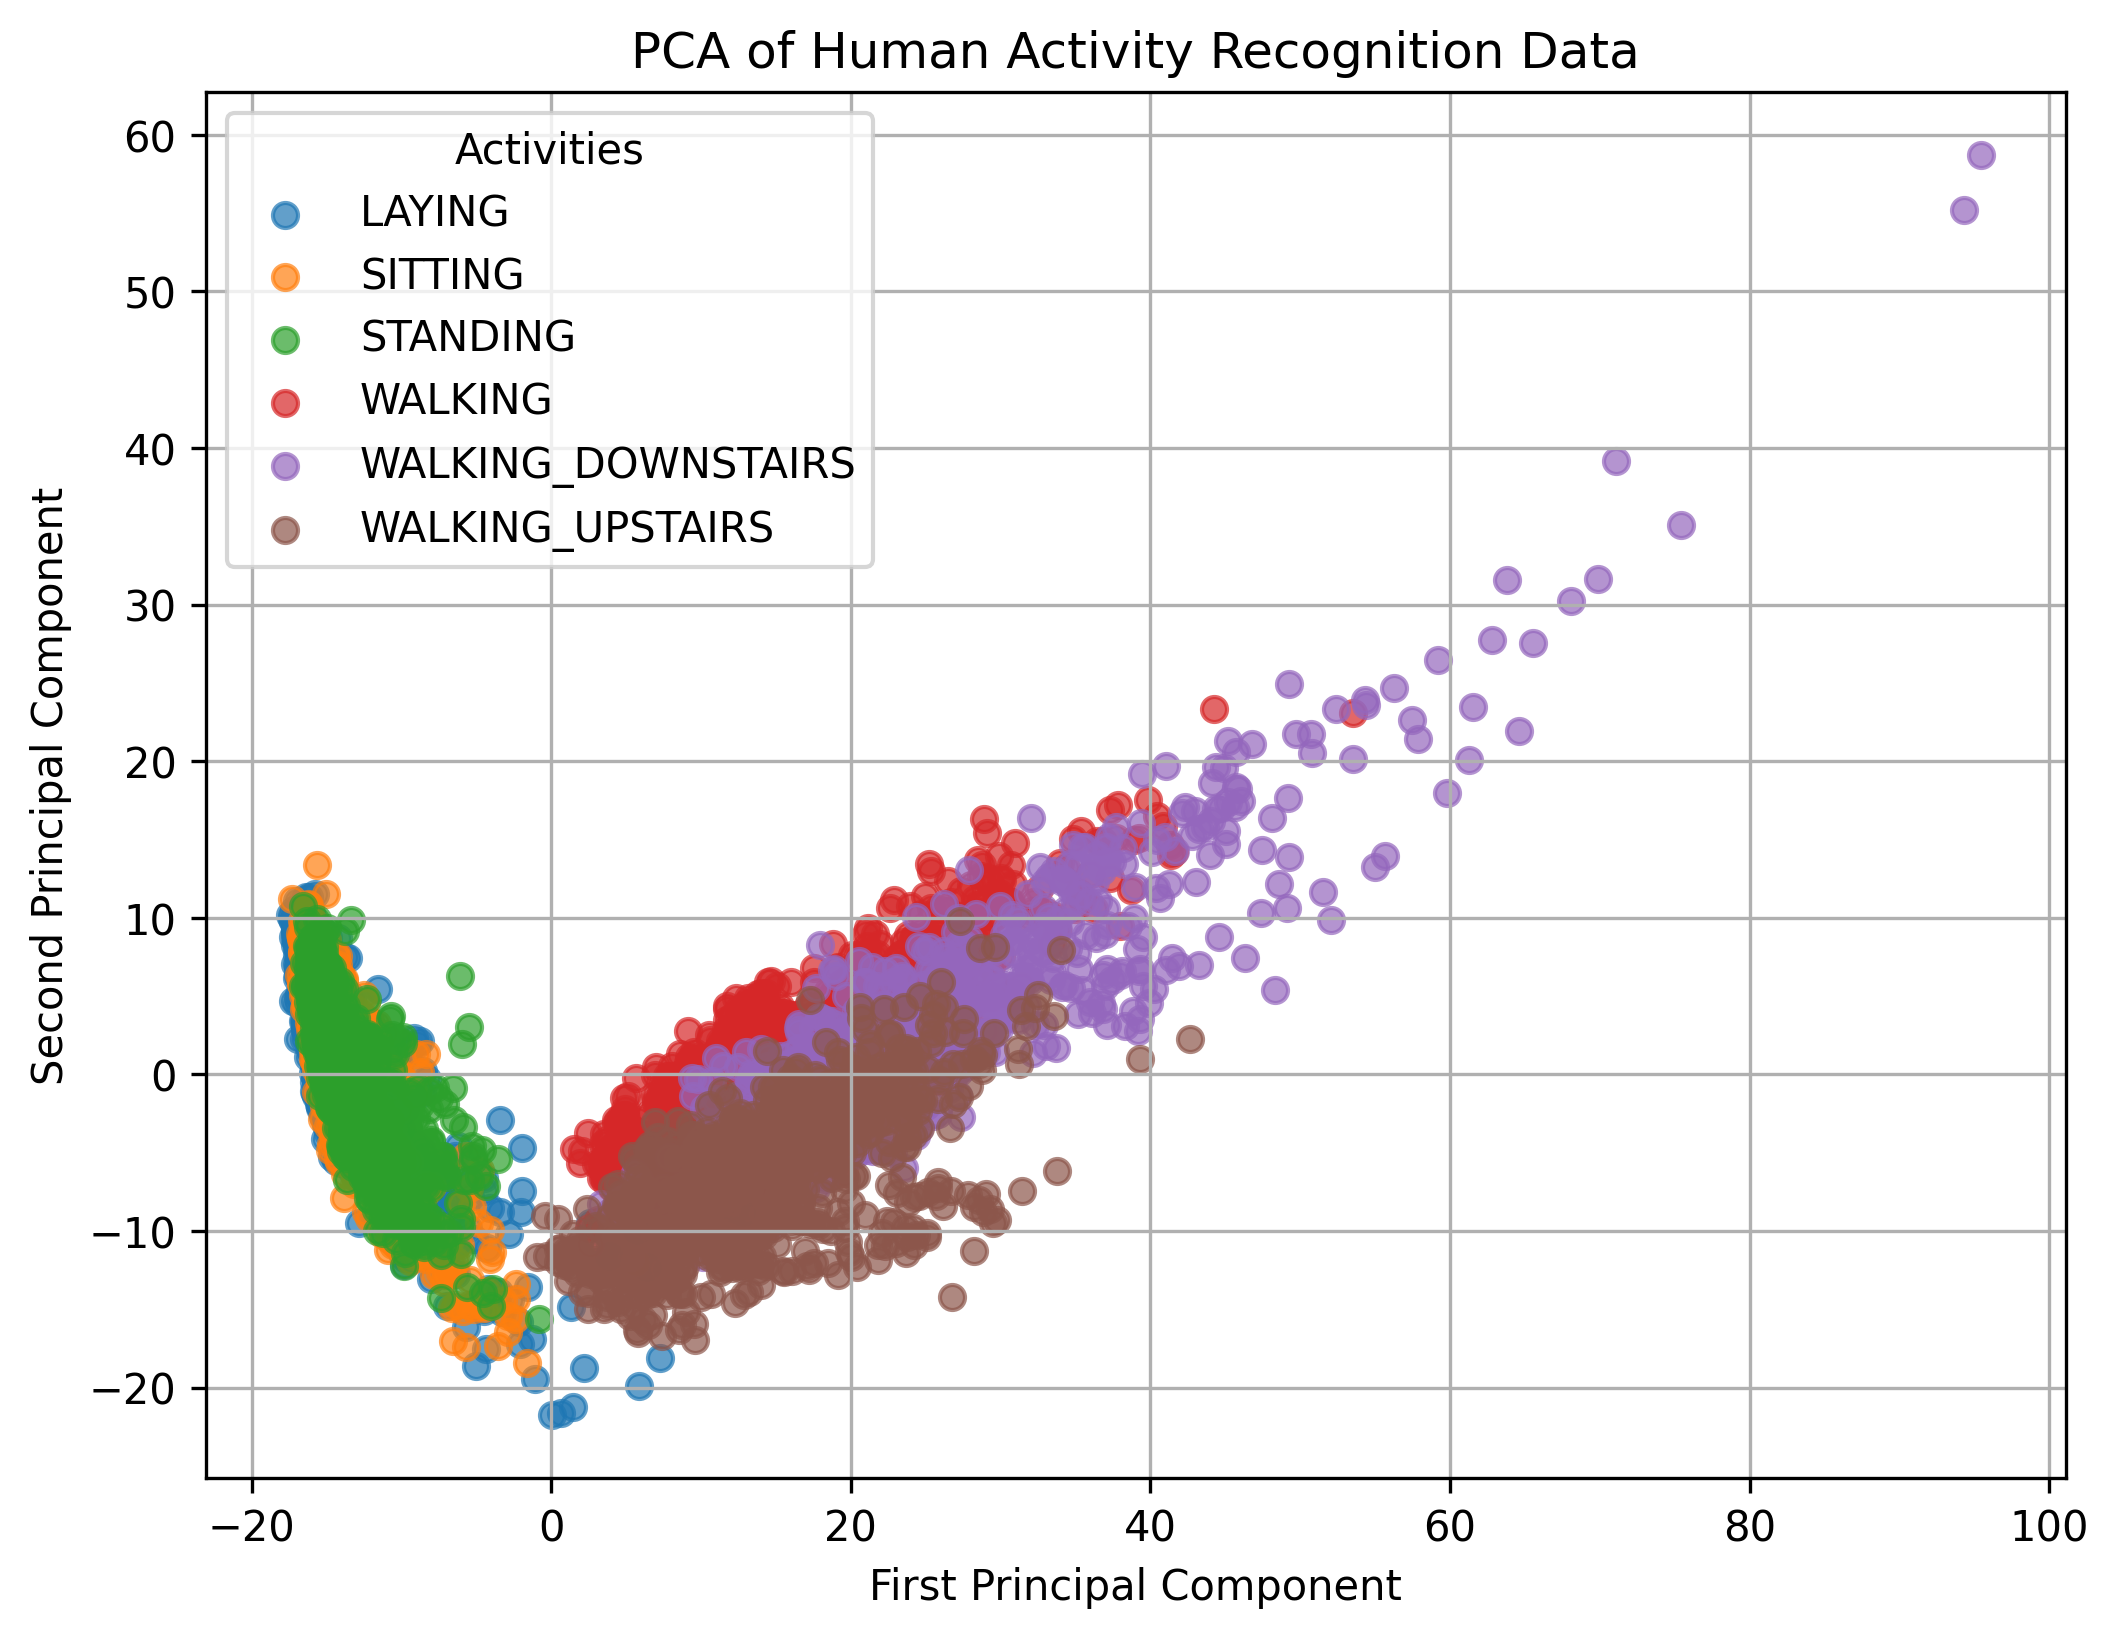
\includegraphics[width=0.85\textwidth]{PCA_activities.png}
    \caption{PCA visualization of Human Activity Recognition training data. Each point represents a sample colored by its activity label.}
    \label{fig:pca-har}
\end{figure}

\end{itemize}

\subsection*{4.2 Choosing The Optimal Number of Clusters [10 points]}
Now we will use K-means clustering (as taught in class) and attempt to choose the optimal number of clusters (k) using two different methods and analyse the results.

\begin{itemize}
\item[a.] Elbow Method:

The Elbow Method is a populer heuristic approach used in K-Means clustering to determine the optimal number of clusters. It provides a systematic way of identifying the best k by analyzing how the distortion (see Question 2) changes as k increases. The distortion is also referred to as inertia, which measures the compactness of clusters.

To determine the optimal k, we plot distortion against k. The curve usually shows a steep drop initially, followed by a slower decline. The ``elbow'' is the point where this change in slope is most pronounced. This 'elbow' point is usually determent from the plot directly but it can also be define mathmatically as the value of k where the second derivative of the distortion is maximized.

Plot the distortion versus k for k = 2 to k = 15. Choose the value of k where the curve sharply flattens (``elbow''), and then create a scatter plot that visualizes the clusters for the chosen k. Each point in the scatter plot should correspond to a data point, with different colors or shapes the different clusters. Use the two principal components you found in part 4.1 as the axes of your plot. In your comments, describe how the distortion changes with increasing k.
\begin{figure}[H]
    \centering
    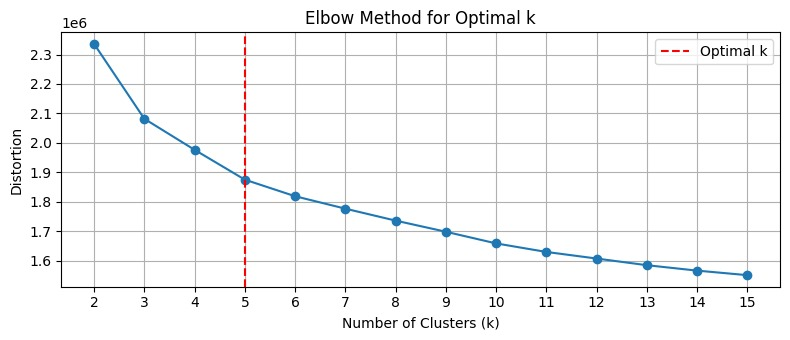
\includegraphics[width=0.85\textwidth]{elbow4.2.jpg}
    \caption{Elbow method plot showing distortion vs. number of clusters (k). The elbow point indicates the optimal number of clusters.}
    \label{fig:elbow-method}
\end{figure}
\begin{figure}[H]
    \centering
    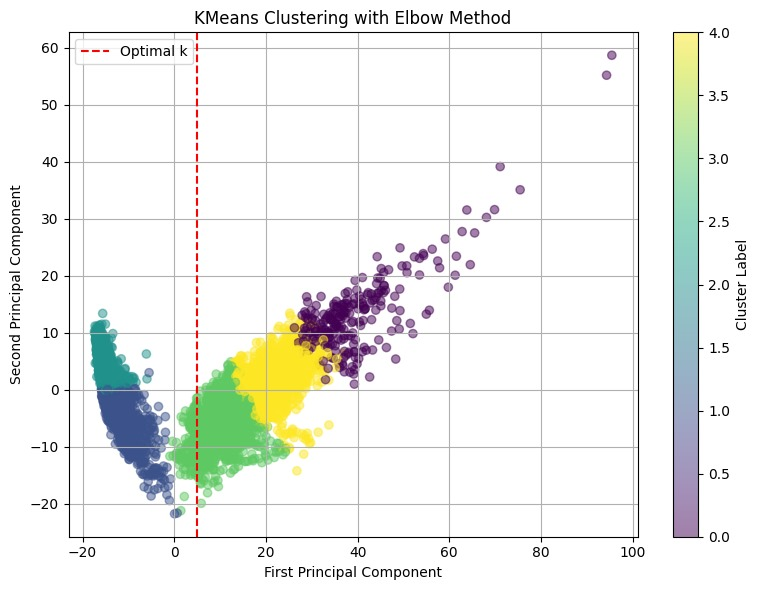
\includegraphics[width=0.85\textwidth]{kmeans4.2.jpg}
    \caption{Scatter plot of clusters obtained from K-means clustering with k = 5. Each point represents a sample colored by its assigned cluster.}
    \label{fig:kmeans-clusters}
\end{figure}
The distortion, which measures the sum of squared distances between data points and their assigned cluster centroids, decreases as the number of clusters (k) increases. This is because adding more clusters allows the centroids to better fit the data, reducing the distance between points and their nearest centroid. However, the rate of decrease in distortion diminishes as k becomes larger, leading to the "elbow" point, where adding more clusters provides diminishing returns in reducing distortion.\\

\item[b.] Adjusted Rand Index (ARI)

The Adjusted Rand Index (ARI) is a clustering evaluation metric that measures the alignment between a predicted clustering and a ground truth labels. In our case, the clustering obtained by K-means and the true activity labels.

The ARI score is normalized so that ARI = 1 indicates perfect clustering (identical to the ground truth), ARI = 0 corresponds to random clustering (no better than chance), and ARI < 0 suggests clustering worse than random assignment\footnote{This suggests that the clustering systematically splits cohesive groups apart, causing ARI to be negative.}.

Compute ARI for k = 2 to k = 15 using the true activity labels. (you can use sklearn adjusted\_rand\_score for this task) Pick the value of k with maximal ARI and describe how the ARI changes with increasing k. Create a scatter plot of the resulting clusters, as you did for the elbow method clusters above.
\begin{figure}[H]
    \centering
    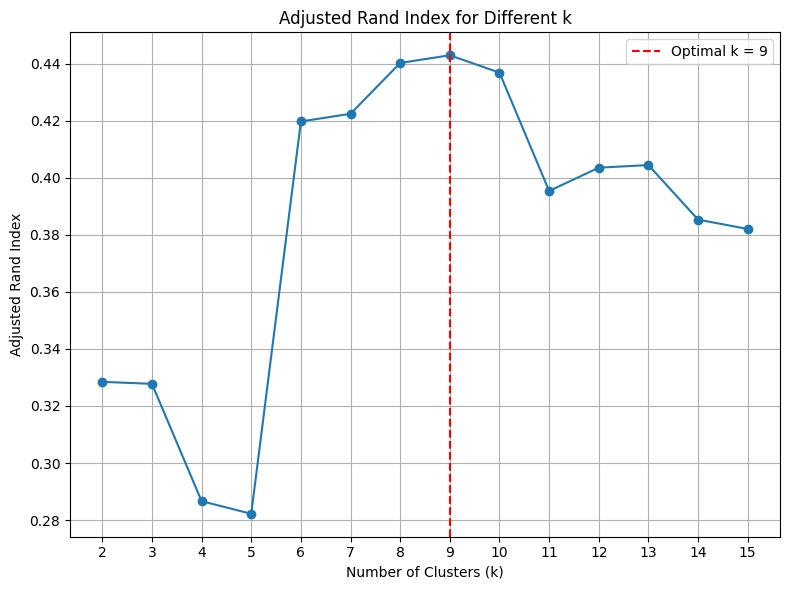
\includegraphics[width=0.85\textwidth]{ari4.2.jpg}
    \caption{Adjusted Rand Index (ARI) vs. number of clusters (k). The maximum ARI indicates the best clustering performance.}
    \label{fig:ari-method}
\end{figure}
\begin{figure}[H]
    \centering
    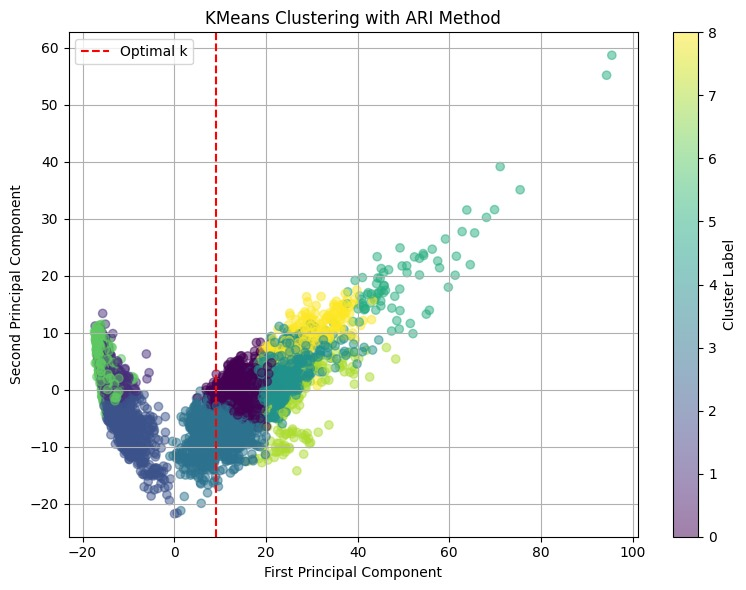
\includegraphics[width=0.85\textwidth]{aricluster4.2.jpg}
    \caption{Scatter plot of clusters obtained from K-means clustering with k = 5, colored by ARI scores.}
    \label{fig:kmeans-clusters-ari}
\end{figure}
The ARI score increases with the number of clusters (k) up to a certain point, indicating that the clustering is becoming more aligned with the true activity labels. However, after reaching a peak, the ARI score may plateau or even decrease slightly as k continues to increase. This suggests that while more clusters can improve clustering performance, there is a point where adding more clusters does not significantly enhance the alignment with the true labels. The optimal k based on ARI is 5, which corresponds to the maximum ARI score of 0.4533.
\end{itemize}

\subsection*{4.3 Prototype Selection using K-means Clustering [10 points]}
Prototype selection refers to the process of choosing a subset of representative data points from a larger dataset to reduce storage, computational cost, and redundancy while preserving essential information for classification or clustering tasks. It can also help reduce labeling time, particularly in scenarios where manual annotation is costly and time-consuming, such as active learning and semi-supervised learning. k-means clustering can be used to select prototypes by selecting prototypes from each of the k identified clusters, thus ensuring a diversity of data in the selected prototypes.

In this section, we will simulate this scenario by limiting the number of labeled samples used to train a logistic regression classifier.

\begin{itemize}
\item[a.] Random Selection: Begin by implementing a uniformly random selection strategy to choose 120 data points from the training data set. After selecting the prototypes, use the resulting dataset to train a logistic regression model, with the activity type as the label, and calculate the accuracy. Repeat this experiment 10 times and report the average accuracy.
\\\\ Average Accuracy with Random Selection over 10 repetitions:\textbf{ 0.9219}
\\

\item[b.] Using K-means Clustering by Class: Now perform k-means clustering on the training dataset using k = 20 for each label independently and identify the cluster centers. Based on these centers, you will then for each cluster centroids choose the closest points as representative training data (you will get 120 points). Use these points to train a logistic regression model. Compare the accuracy of the new model to the one trained in part (a) to assess how using clustering for prototype selection affects the performance.
\\\\ Accuracy with K-means Selection: \textbf{0.8931}\\
\end{itemize}
Using clustering for prototype selection slightly reduces the model's performance compared to random selection. This could be due to the loss of diversity in the selected prototypes, as clustering focuses on centroids rather than capturing the full variability of the data.

\subsection*{4.4 Autoencoder for Feature Learning [15 points]}
In this section, we will implement an autoencoder, a type of neural network used for unsupervised learning of efficient codings. Autoencoders work by encoding input data into a lower-dimensional representation and then decoding it back to the original input (see Fig. 2). This process forces the network to learn a compressed representation of the data.

Autoencoders are particularly useful for dimensionality reduction, feature extraction, and denoising. In this part of the problem, we will leverage an autoencoder to create a more compact and more informative representation of the raw sensor data from the Human Activity Recognition dataset by training an autoencoder on the raw sensor readings.

This question will provide you with hands-on experience using PyTorch to build and train and implementing a bidirectional GRU autoencoder neural network.

\begin{figure}[h]
\centering
\caption{Image showing autoencoder structure [Source Wikipedia].}
\end{figure}

\begin{itemize}
\item[a.] Create Dataset Class: Begin by loading the raw sensor data as described in the README.txt file. Ensure the data is correctly formatted for input into the autoencoder. Create a PyTorch Dataset class to efficiently load and batch the raw sensor data. Utilize a DataLoader to create batches for training the autoencoder.

\item[b.] Autoencoder Implementation: Implement the TimeSeriesAE autoencoder model using PyTorch. This model should use GRU layers for both the encoder and decoder and an embedding of size 64. Instantiate the model, define an appropriate loss function, and choose an optimizer. Train the autoencoder for 10 epochs. Plot the training loss vs. epochs.
\begin{figure}[H]
    \centering
    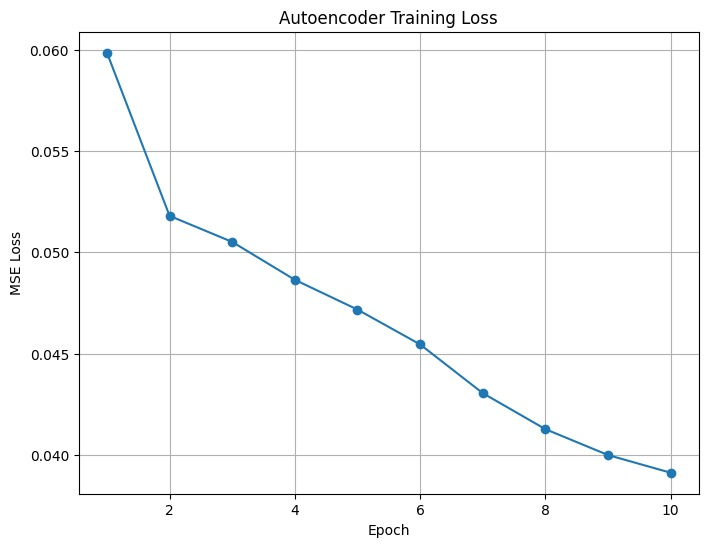
\includegraphics[width=0.85\textwidth]{autoencoderloss.jpg}
    \caption{Training loss vs. epochs for the autoencoder model.}
    \label{fig:autoencoder-loss}
\end{figure}

\item[c.] Embedding Extraction and Visualization: Extract the encoded representations (embeddings) from the trained autoencoder for the training data. To do this, pass the training data through the encoder part of the autoencoder model. Use the first two embeddings to create a scatter plot of the embeddings, colored by the activity labels. Include this plot in your solution PDF.
\begin{figure}[H]
    \centering
    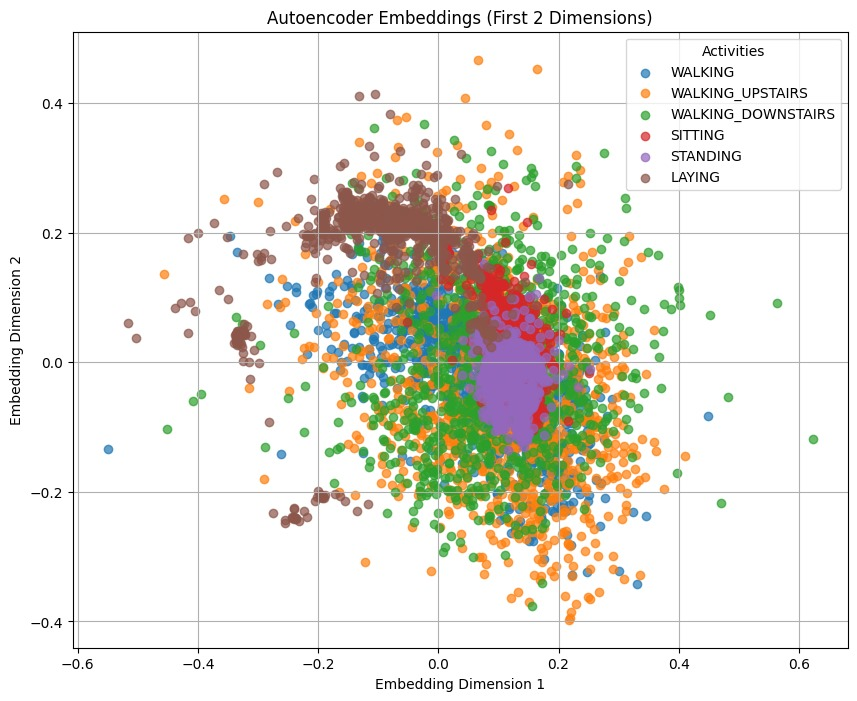
\includegraphics[width=0.85\textwidth]{embeddings.jpg}
    \caption{Scatter plot of the first two embeddings extracted from the autoencoder, colored by activity labels.}
    \label{fig:autoencoder-embeddings}
\end{figure}

\item[d.] Clustering Evaluation and Comparison: Perform K-means clustering on the extracted 64D embeddings. Evaluate the clustering performance using the Adjusted Rand Index (ARI) by comparing the cluster labels with the true activity labels. Compare the ARI obtained by clustering the autoencoder embeddings with the clustering performance you obtained from the hand-engineered features in Part 4.2. Discuss which of the two provides the highest ARI and the potential reasons for that.
\\\\ The ARI obtained by clustering the autoencoder embeddings is 0.4046, while the ARI obtained from the hand-engineered features is 0.4533. The hand-engineered features provide a slightly higher ARI compared to the autoencoder embeddings. 

This difference could be attributed to the fact that the hand-engineered features are specifically designed to capture domain-specific characteristics of the data, which may align better with the ground truth labels. On the other hand, the autoencoder learns a representation in an unsupervised manner, which might not perfectly align with the clustering structure defined by the labels. However, the autoencoder embeddings still perform reasonably well, demonstrating their ability to capture meaningful patterns in the data.
\end{itemize}

\end{enumerate}

\end{document}